\section{编程模型}
\label{sec:prog-model}

\begin{frame}
  \begin{center}
    \Huge{\textcolor{red}{编程模型}}
  \end{center}

  \begin{enumerate}
    \item \alert{计算图}
    \item \alert{变量}
    \item \alert{会话}
    \item \alert{图构造与执行}    
  \end{enumerate}     
\end{frame}

\subsection{计算图}

\begin{frame}{$ Graph = Set\{OP\} + Set\{Tensor\} $}
  \begin{figure}
    \centering
    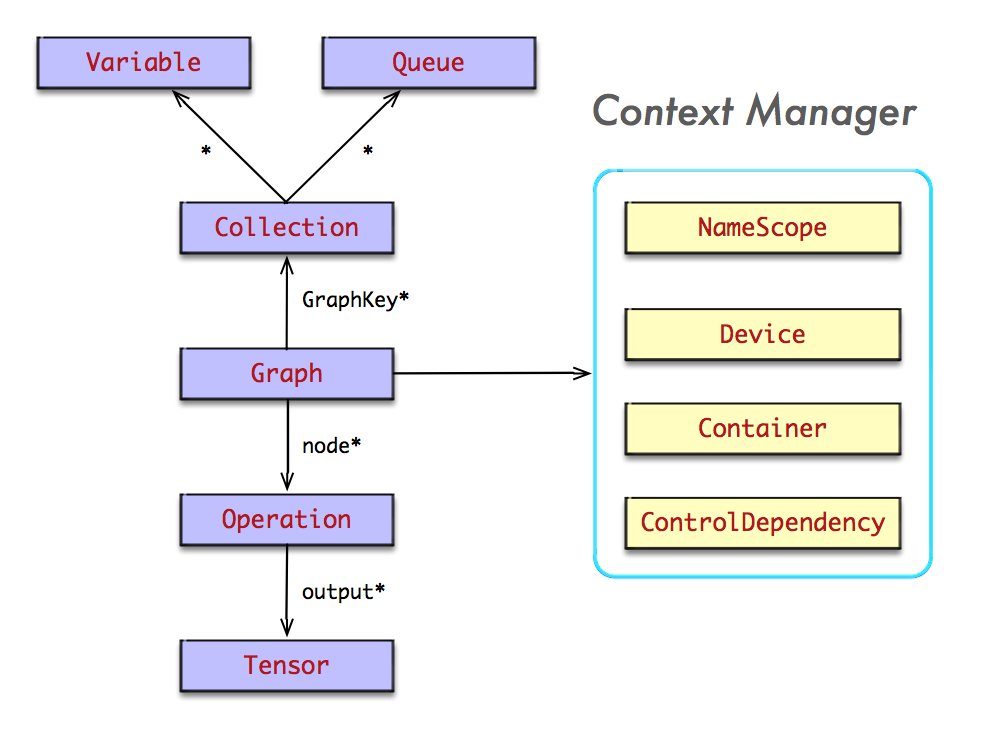
\includegraphics[width=0.8\textwidth]{py-graph-model.png}
  \end{figure}
\end{frame}

\begin{frame}{OP: 抽象计算}
  \begin{figure}
    \centering
    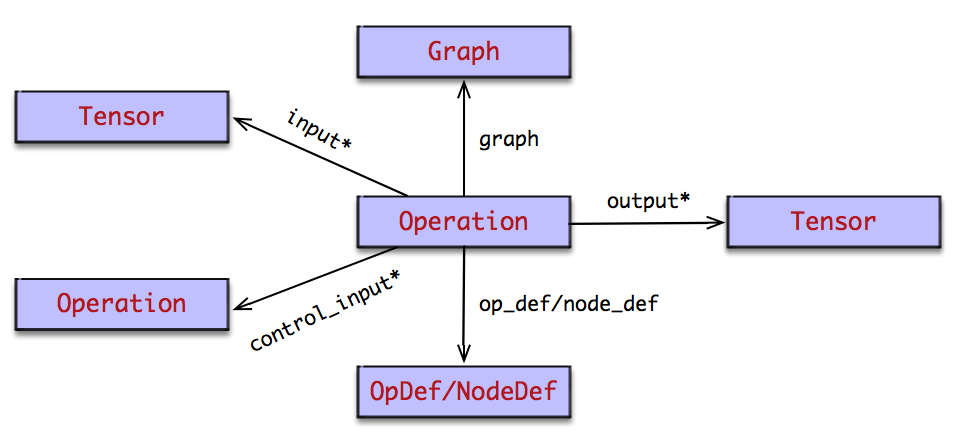
\includegraphics[width=0.8\textwidth]{py-op-model.png}
  \end{figure}
\end{frame}

\begin{frame}{Tensor: 承载数据}
  \begin{figure}
    \centering
    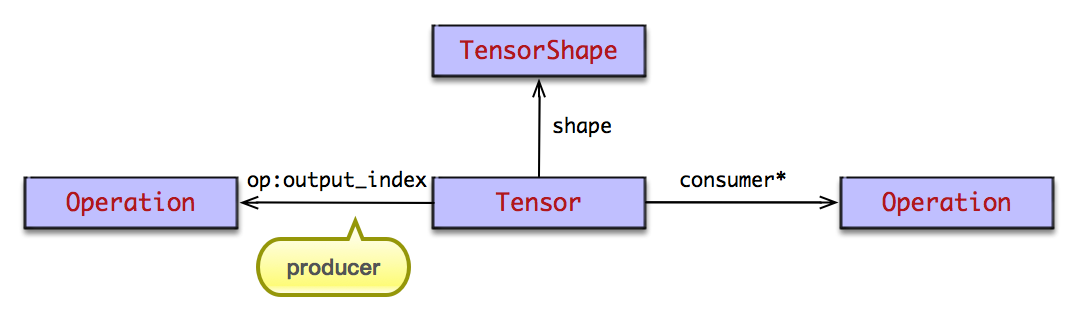
\includegraphics[width=0.8\textwidth]{py-tensor-model.png}
  \end{figure}
\end{frame}

\begin{frame}{有向边}
  \begin{block}{两种类型}
    \begin{itemize}
      \item \alert{普通边}: 承载Tensor,且表示执行依赖关系
      \item \alert{控制依赖边}: 不承载Tensor,仅表示执行依赖关系  
    \end{itemize}
  \end{block}
\end{frame}

\subsection{变量}

\begin{frame}{初始化模型}
  \begin{figure}
    \centering
    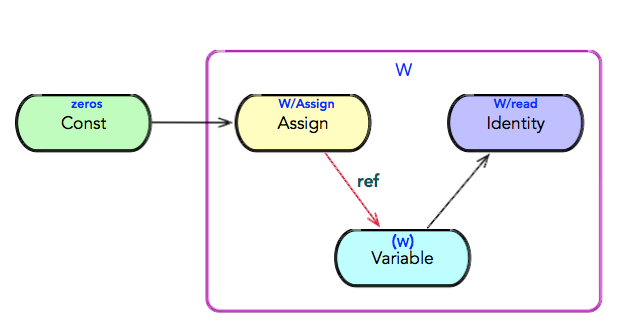
\includegraphics[width=0.8\textwidth]{variable-initialization-model.png}
  \end{figure}
\end{frame}

\begin{frame}{探秘init\_op}
  \begin{figure}
    \centering
    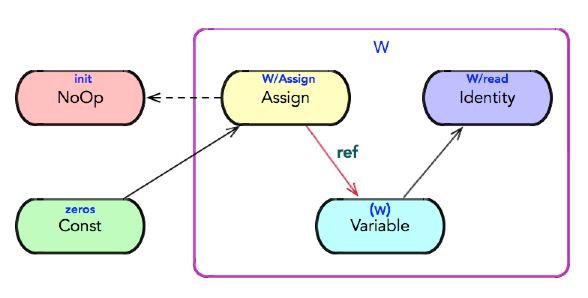
\includegraphics[width=0.75\textwidth]{variable-initialization-no-op.png}
  \end{figure}
\end{frame}

\begin{frame}{初始化依赖}
  \begin{figure}
    \centering
    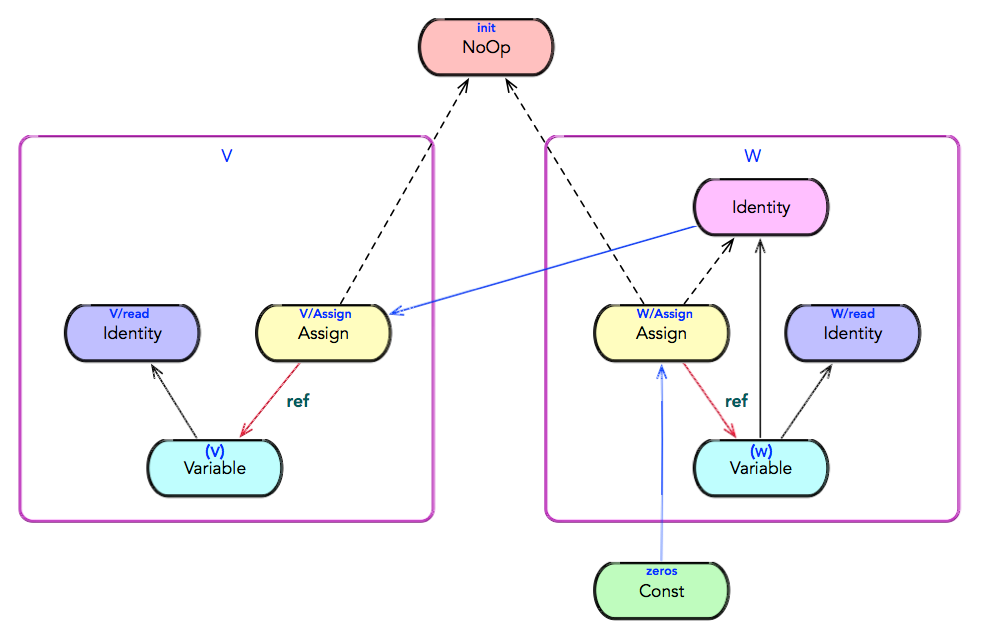
\includegraphics[width=0.9\textwidth]{variable-initialization-dependency.png}
  \end{figure}
\end{frame}

\subsection{会话}

\begin{frame}{生命周期: Python}
  \begin{figure}
    \centering
    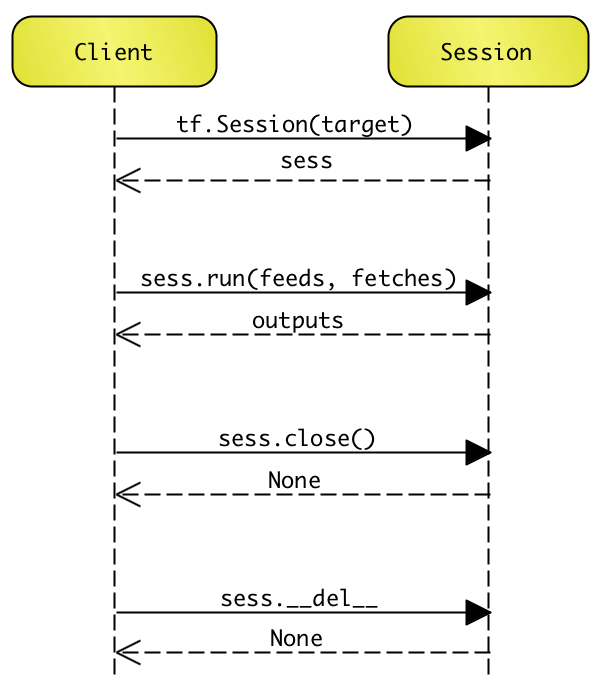
\includegraphics[width=0.52\textwidth]{py-session-lifecycle.png}
  \end{figure}
\end{frame}

\begin{frame}{生命周期: C++}
  \begin{figure}
    \centering
    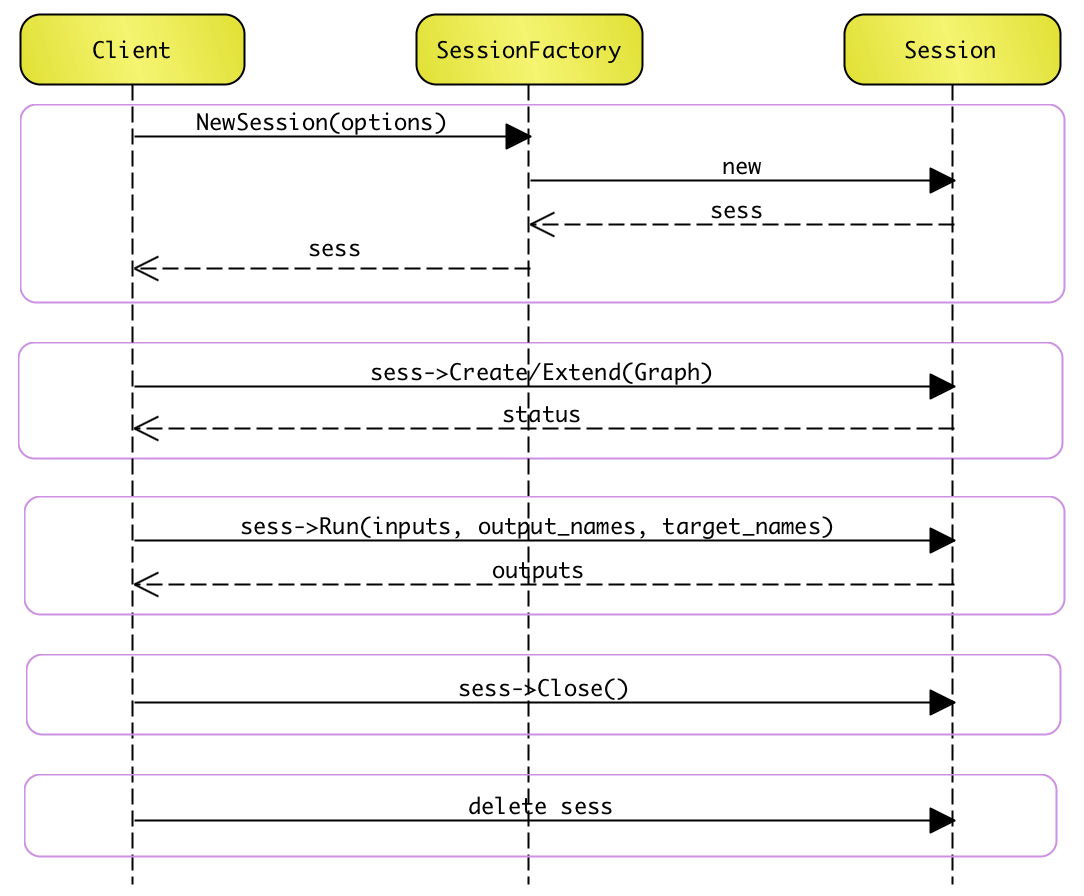
\includegraphics[width=0.7\textwidth]{cc-session-lifecycle.png}
  \end{figure}
\end{frame}

\subsection{图构造与执行}

\begin{frame}{图构造与传递}
  \begin{figure}
    \centering
    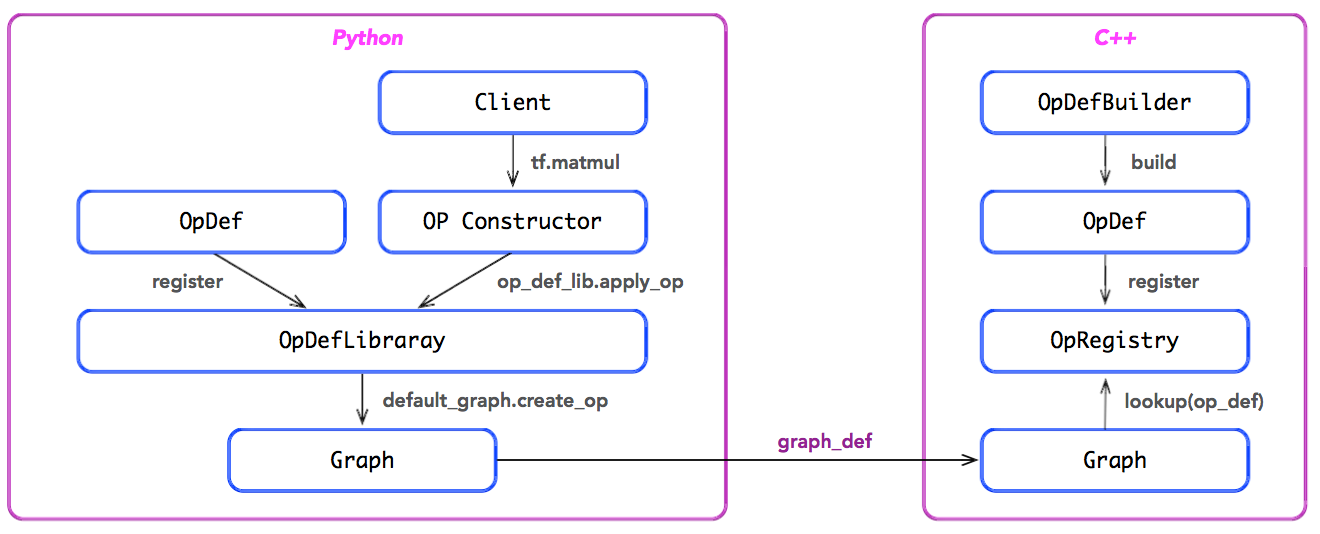
\includegraphics[width=0.95\textwidth]{py-graph-creation.png}
  \end{figure}
\end{frame}

\begin{frame}{实例: OP构造器}
  \begin{figure}
    \centering
    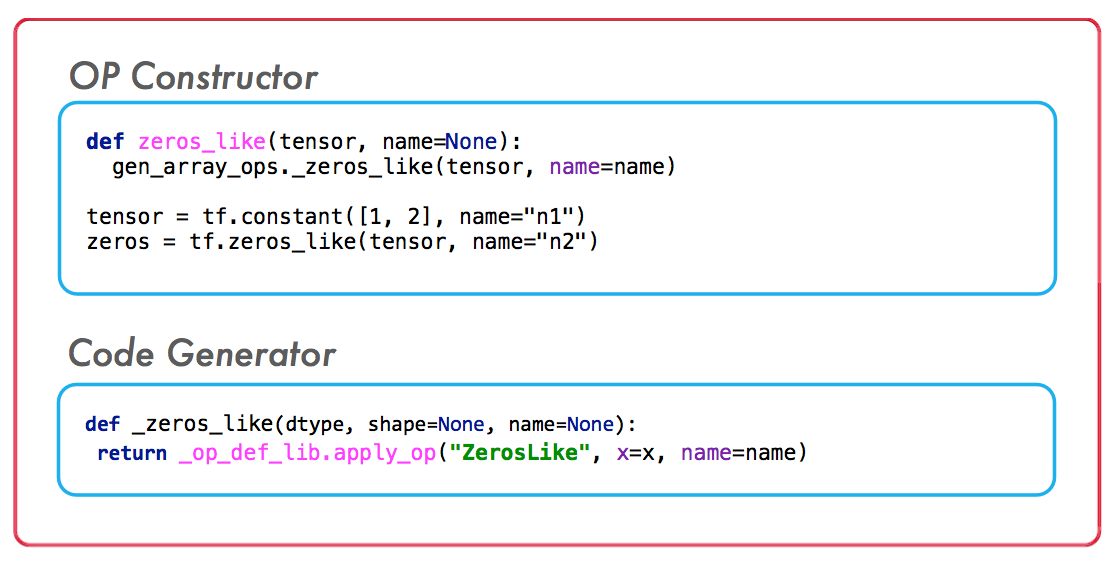
\includegraphics[width=0.9\textwidth]{py-graph-construction-example-1.png}
  \end{figure}
\end{frame}

\begin{frame}{实例: 构造OP}
  \begin{figure}
    \centering
    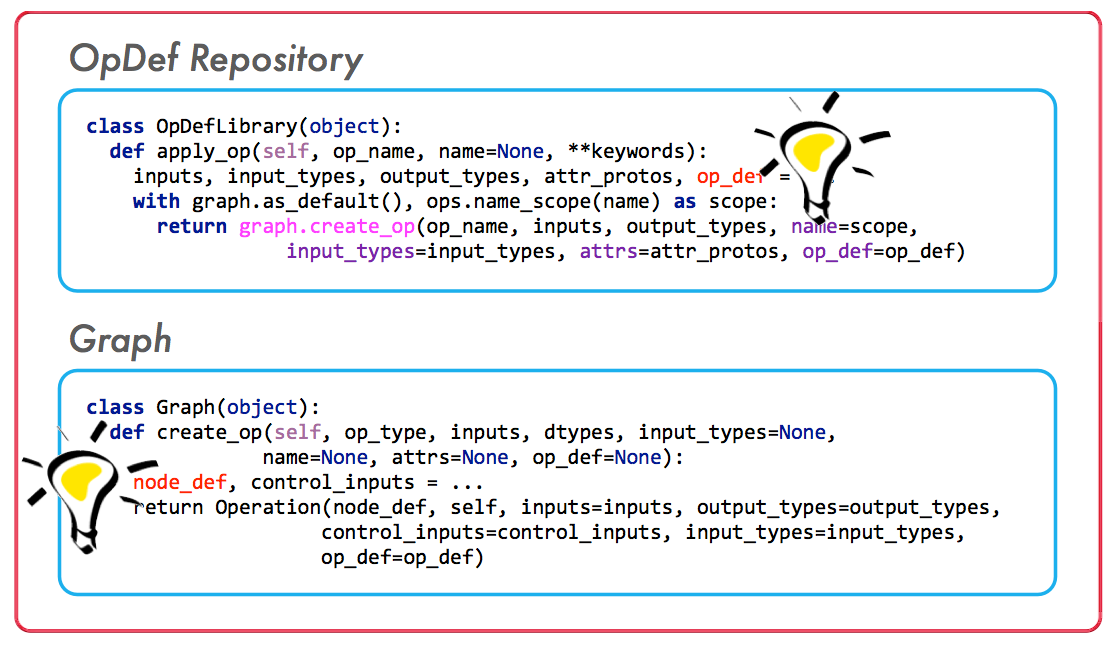
\includegraphics[width=0.9\textwidth]{py-graph-construction-example-2.png}
  \end{figure}
\end{frame}

\begin{frame}{实例: 图构造}
  \begin{figure}
    \centering
    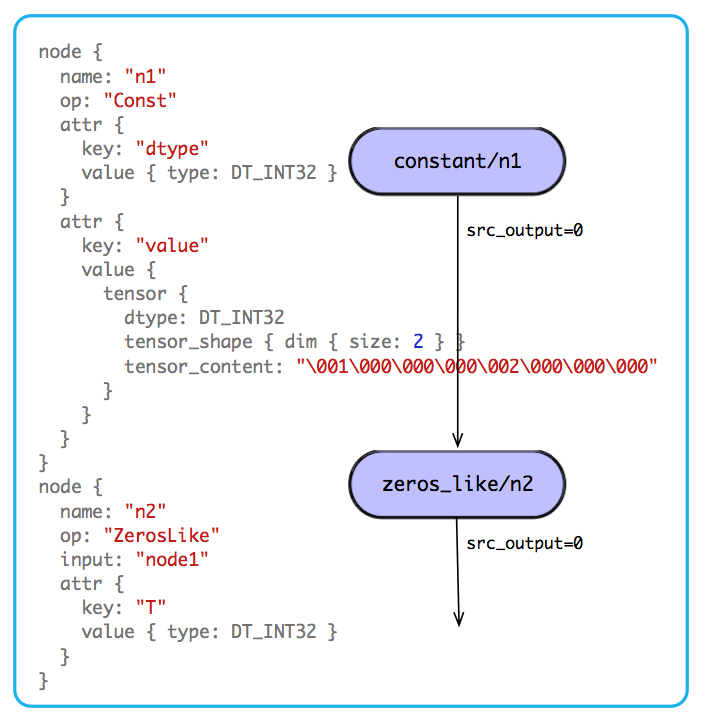
\includegraphics[width=0.59\textwidth]{py-graph-construction-example-3.png}
  \end{figure}
\end{frame}

\begin{frame}{实例:图执行}
  \begin{figure}
    \centering
    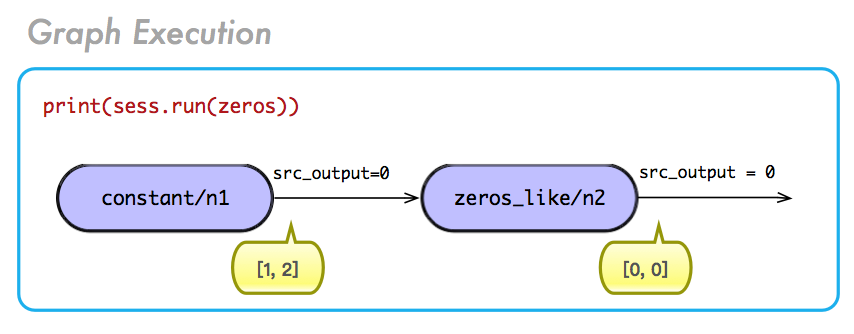
\includegraphics[width=0.8\textwidth]{py-graph-execution.png}
  \end{figure}
\end{frame}
